\section*{Unidad 6: Series y sucesiones}
\addcontentsline{toc}{section}{\protect\numberline{}Unidad 6: Series y sucesiones}%

\subsection*{Actividad 1.A}

En primer lugar, completamos la tabla con las combinaciones posibles
para construir la pared con los largos deseados:

\begin{center}
    \begin{tabular}{ c c c c c c c c c c c c }
        Cantidad de ladrillos   & 1 & 2 & 3 & 4 & 5 & 6 & 7 & 8 & 9 \\
        \hline                  &                                   \\ [-1em]
        N\(^{\circ}\) de formas & 1 & 2 & 3 &   &   &   &   &   &   \\
        \hline
    \end{tabular}
\end{center}

En un primer momento, parecería que, siendo \(a_{1}=1\),
y \(a_{2}=2\), definiendo la sucesión por recurrencia podríamos decir que
\(a_n = a_{n-1} + a_{n-2}\).
Probamos las combinaciones posibles para una pared de largo 4:

\begin{center}
    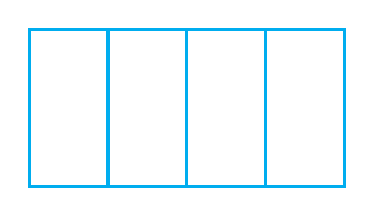
\begin{tikzpicture}
        \draw[cyan, very thick] (0,0) rectangle (1,2);
        \draw[cyan, very thick] (1,0) rectangle (2,2);
        \draw[cyan, very thick] (2,0) rectangle (3,2);
        \draw[cyan, very thick] (3,0) rectangle (4,2);
    \end{tikzpicture}
\end{center}

\begin{center}
    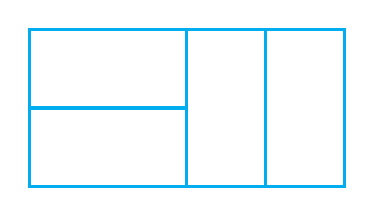
\begin{tikzpicture}
        \draw[cyan, very thick] (0,0) rectangle (2,1);
        \draw[cyan, very thick] (0,1) rectangle (2,2);
        \draw[cyan, very thick] (2,0) rectangle (3,2);
        \draw[cyan, very thick] (3,0) rectangle (4,2);
    \end{tikzpicture}
\end{center}

\begin{center}
    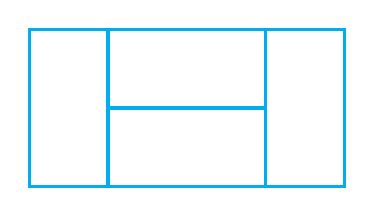
\begin{tikzpicture}
        \draw[cyan, very thick] (0,0) rectangle (1,2);
        \draw[cyan, very thick] (1,0) rectangle (3,1);
        \draw[cyan, very thick] (1,1) rectangle (3,2);
        \draw[cyan, very thick] (3,0) rectangle (4,2);
    \end{tikzpicture}
\end{center}

\begin{center}
    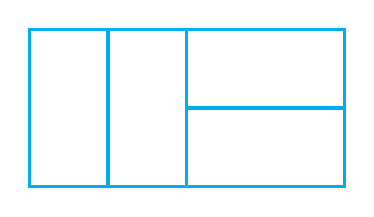
\begin{tikzpicture}
        \draw[cyan, very thick] (0,0) rectangle (1,2);
        \draw[cyan, very thick] (1,0) rectangle (2,2);
        \draw[cyan, very thick] (2,0) rectangle (4,1);
        \draw[cyan, very thick] (2,1) rectangle (4,2);
    \end{tikzpicture}
\end{center}

\begin{center}
    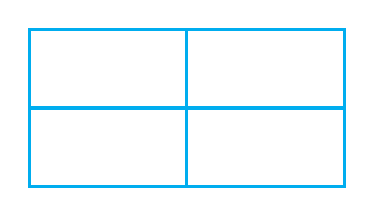
\begin{tikzpicture}
        \draw[cyan, very thick] (0,0) rectangle (2,1);
        \draw[cyan, very thick] (0,1) rectangle (2,2);
        \draw[cyan, very thick] (2,0) rectangle (4,1);
        \draw[cyan, very thick] (2,1) rectangle (4,2);
    \end{tikzpicture}
\end{center}

Como observamos en los diagramas,
la sucesión cumple con \(a_n = a_{n-1} + a_{n-2}\),
por lo tanto:

\begin{center}
    \begin{tabular}{ c c c c c c c c c c c c }
        Cantidad de ladrillos   & 1 & 2 & 3 & 4 & 5 & 6  & 7  & 8  & 9  \\
        \hline                  &                                       \\ [-1em]
        N\(^{\circ}\) de formas & 1 & 2 & 3 & 5 & 8 & 13 & 21 & 34 & 55 \\
        \hline
    \end{tabular}
\end{center}

Observamos que el número de formas sigue la sucesión de Fibonacci,
desde su tercer elemento -incluído- en adelante.
Esto es esperable, puesto que comparten la misma definición por recurrencia:
\(a_n = a_{n-1} + a_{n-2}\).
Solo que en el caso del problema que estamos tratando, \(a_{1} = 1\) y 
\(a_{2} = 2\), mientras que en Fibonacci \(a_{1} = 0\) \(a_{2} = 1\),
por ello hay un desplazamiento en los términos y nuestra sucesión comienza por 
el tercer término de Fibonacci.